\documentclass[12pt]{article}

\usepackage[utf8]{inputenc}
\usepackage{amsmath, amssymb, amsfonts, cancel}
\usepackage{graphicx}
\usepackage[letterpaper, left=1in, right=1in, top=1in, bottom=1in]{geometry}
\usepackage{booktabs}
\usepackage{multirow}
\usepackage{float}
\usepackage{caption}
\usepackage{colortbl}
\usepackage{xcolor}
\definecolor{paleYellow}{RGB}{255,255,180}
\usepackage{physics}
\usepackage{hyperref}
\usepackage[spanish]{babel}

\title{
Práctica 8: HSRP\\[0.5em]
\large Administración de redes
}

\author{
Jorge Alberto Suarez Saldana\\
\small Matrícula: 355992\\
\small Profesor: Raymundo Antonio González Grimaldo
}

\date{\today}

\begin{document}
\maketitle

\section{Objetivo}
El objetivo de esta práctica es configurar el protocolo \textbf{HSRP (Hot Standby Router Protocol)} para proporcionar redundancia en la puerta de enlace predeterminada dentro de una red LAN. Asimismo, se busca verificar su funcionamiento ante fallas de conectividad.

\section{Marco Teórico}

El protocolo HSRP es un protocolo de redundancia de primer salto (FHRP) que permite a varios routers actuar como un único router virtual. Esto se logra mediante una dirección IP y MAC virtual compartida.

\begin{itemize}
    \item \textbf{Router activo:} Maneja el tráfico.
    \item \textbf{Router en espera:} Toma el control si el activo falla.
    \item \textbf{IP virtual:} Puerta de enlace usada por los hosts.
\end{itemize}

\section{Desarrollo}

\subsection{Parte 1: Verificación de conectividad}

Se realizaron pruebas con el comando:

\begin{verbatim}
tracert 209.165.200.226
\end{verbatim}

\textbf{Resultados:}
\begin{itemize}
    \item Desde PC-A: La ruta pasa por R1 hacia Internet.
    \item Desde PC-B: La ruta pasa por R3 hacia Internet.
\end{itemize}

Al desconectar R3:
\begin{itemize}
    \item PC-B pierde conectividad hacia el servidor.
\end{itemize}

\subsection{Parte 2: Configuración de HSRP}

\subsubsection{Configuración en R1 (Activo)}

\begin{verbatim}
interface g0/1
 standby version 2
 standby 1 ip 192.168.1.254
 standby 1 priority 150
 standby 1 preempt
\end{verbatim}

\subsubsection{Configuración en R3 (Standby)}

\begin{verbatim}
interface g0/0
 standby version 2
 standby 1 ip 192.168.1.254
\end{verbatim}

\textbf{Observaciones:}
\begin{itemize}
    \item R1 tiene prioridad 150 (activo).
    \item R3 mantiene prioridad por defecto 100 (standby).
\end{itemize}

\subsection{Verificación}

Comando utilizado:

\begin{verbatim}
show standby
\end{verbatim}

\textbf{Resultados:}
\begin{itemize}
    \item Router activo: R1
    \item IP virtual: 192.168.1.254
    \item MAC virtual: 0000.0C9F.F001
    \item Router standby: R3 (192.168.1.3, prioridad 100)
\end{itemize}

\subsection{Cambio de Gateway}

Se actualizó el gateway de todos los dispositivos a:

\begin{center}
\textbf{192.168.1.254}
\end{center}

\textbf{Resultado:}  
Los pings al servidor fueron exitosos.

\section{Parte 3: Pruebas de Fallo}

\subsection{Fallo del router activo}

Al desconectar R1:
\begin{itemize}
    \item R3 toma el rol activo.
    \item Se observa un pequeño retraso durante la conmutación.
    \item La conectividad se restablece automáticamente.
\end{itemize}

\subsection{Restauración}

Al reconectar R1:
\begin{itemize}
    \item Gracias a \textbf{preempt}, R1 retoma el rol activo.
    \item La ruta original se restablece.
\end{itemize}

\section{Resultados}

\begin{itemize}
    \item HSRP proporciona alta disponibilidad.
    \item Los hosts no requieren reconfiguración.
    \item La red tolera fallos de gateway sin interrupción significativa.
\end{itemize}

    \begin{figure}[H]
  \centering
  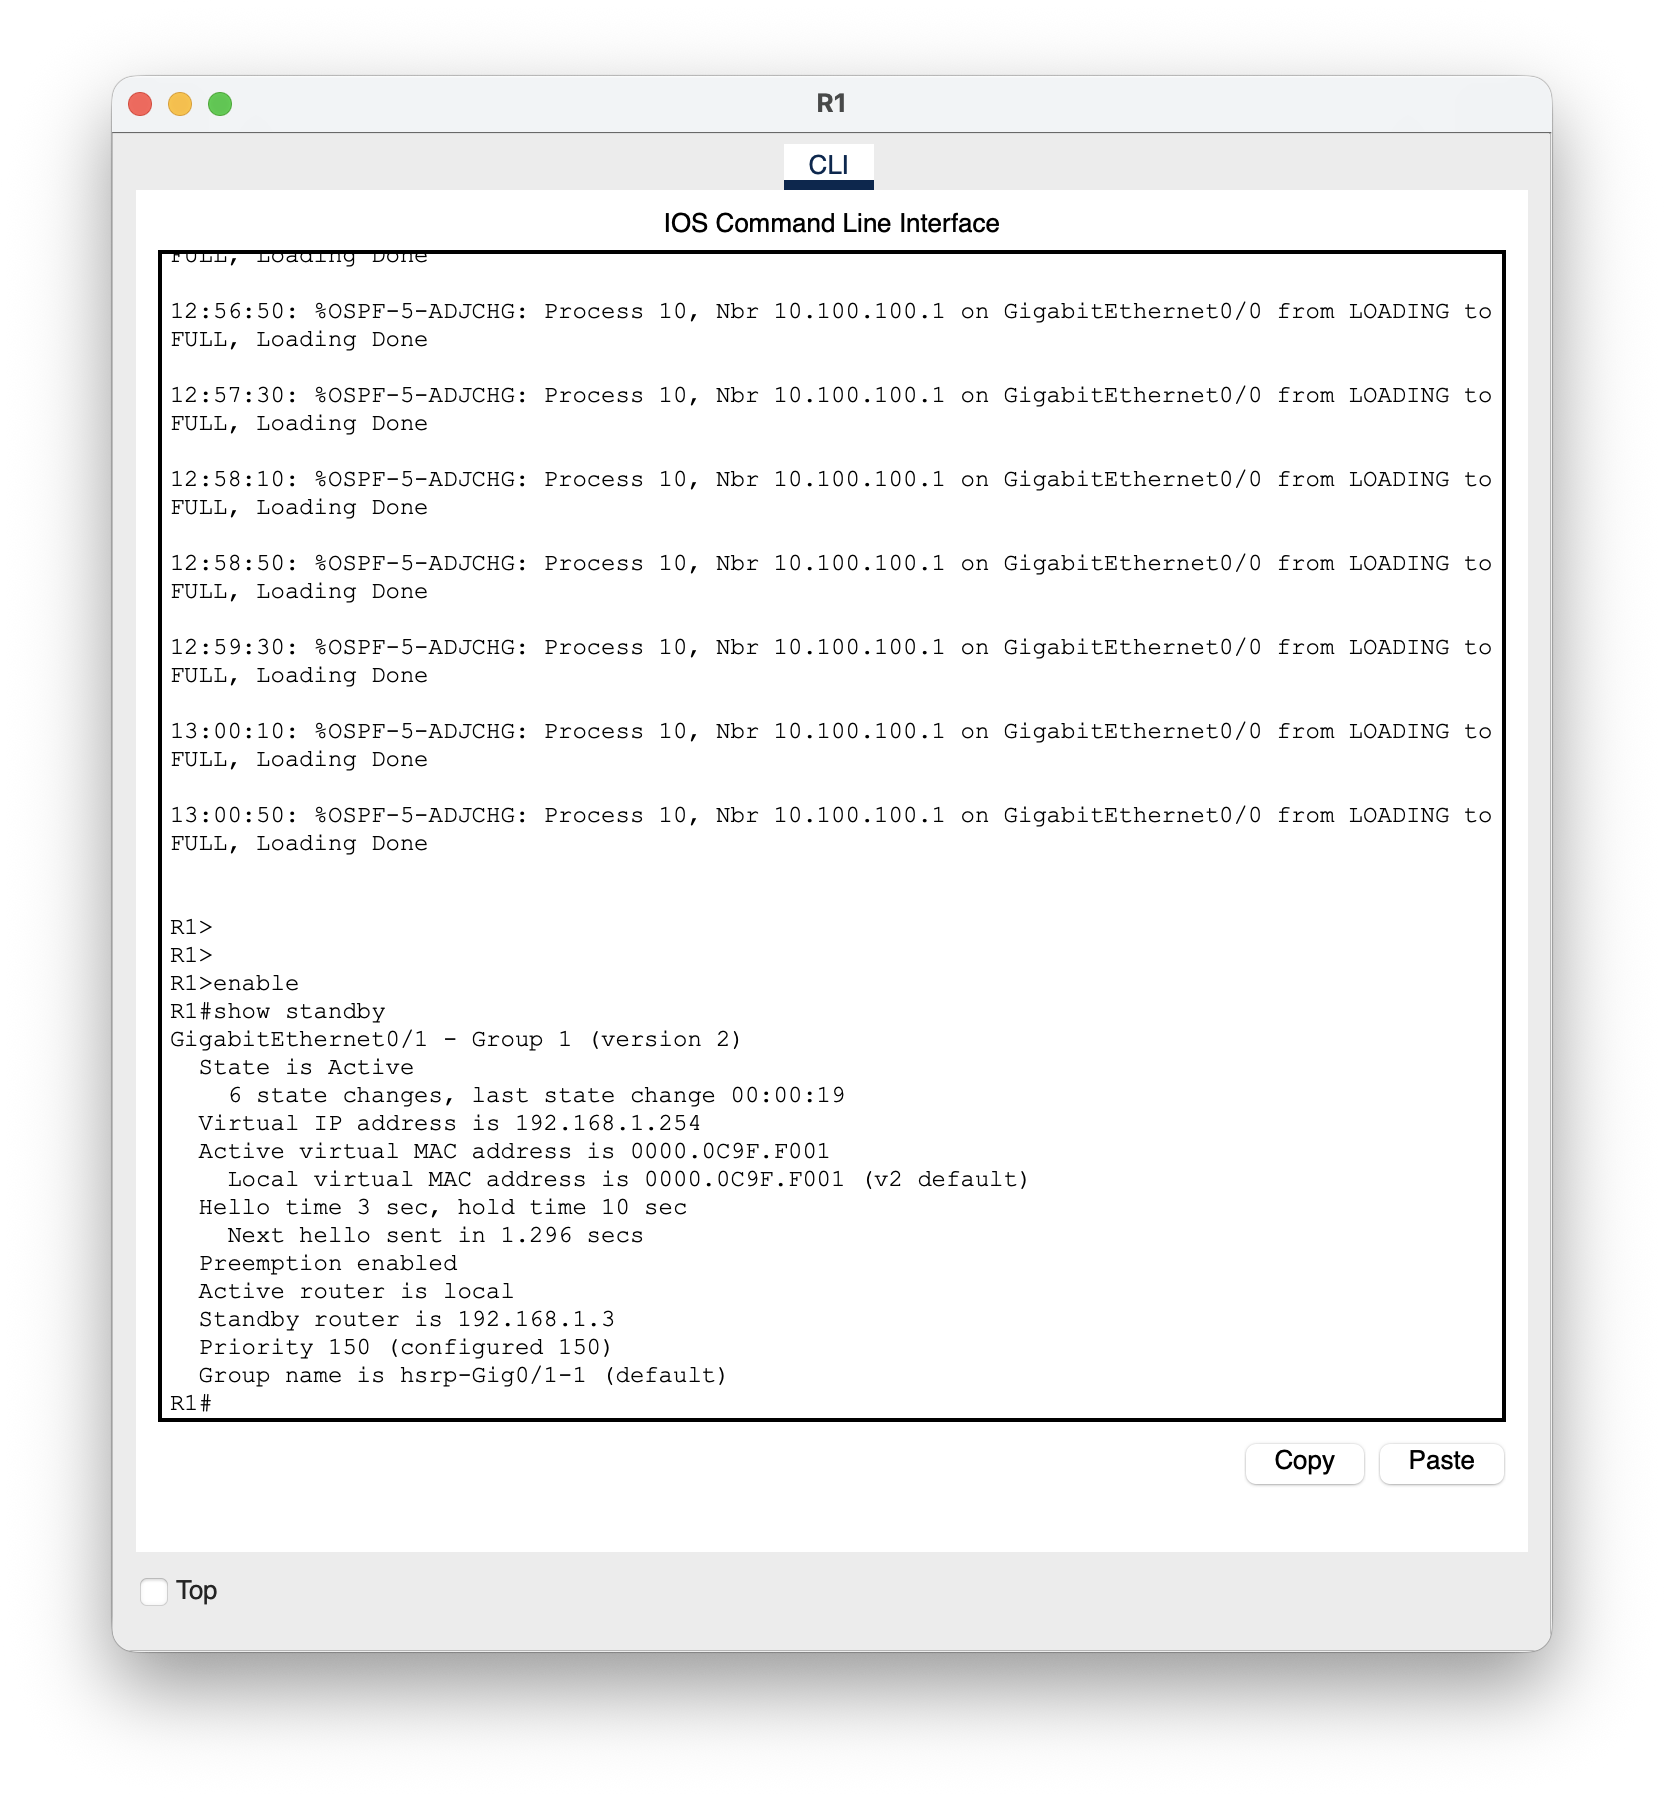
\includegraphics[width=0.8\textwidth]{showStandbyR1.png}
  \caption{Comando show standby en R1}\label{fig:showStandbyR1}
\end{figure}

    \begin{figure}[H]
  \centering
  \includegraphics[width=0.8\textwidth]{showStandbyR3.png}
  \caption{Comando show standby en R3}\label{fig:showStandbyR3}
\end{figure}

    \begin{figure}[H]
  \centering
  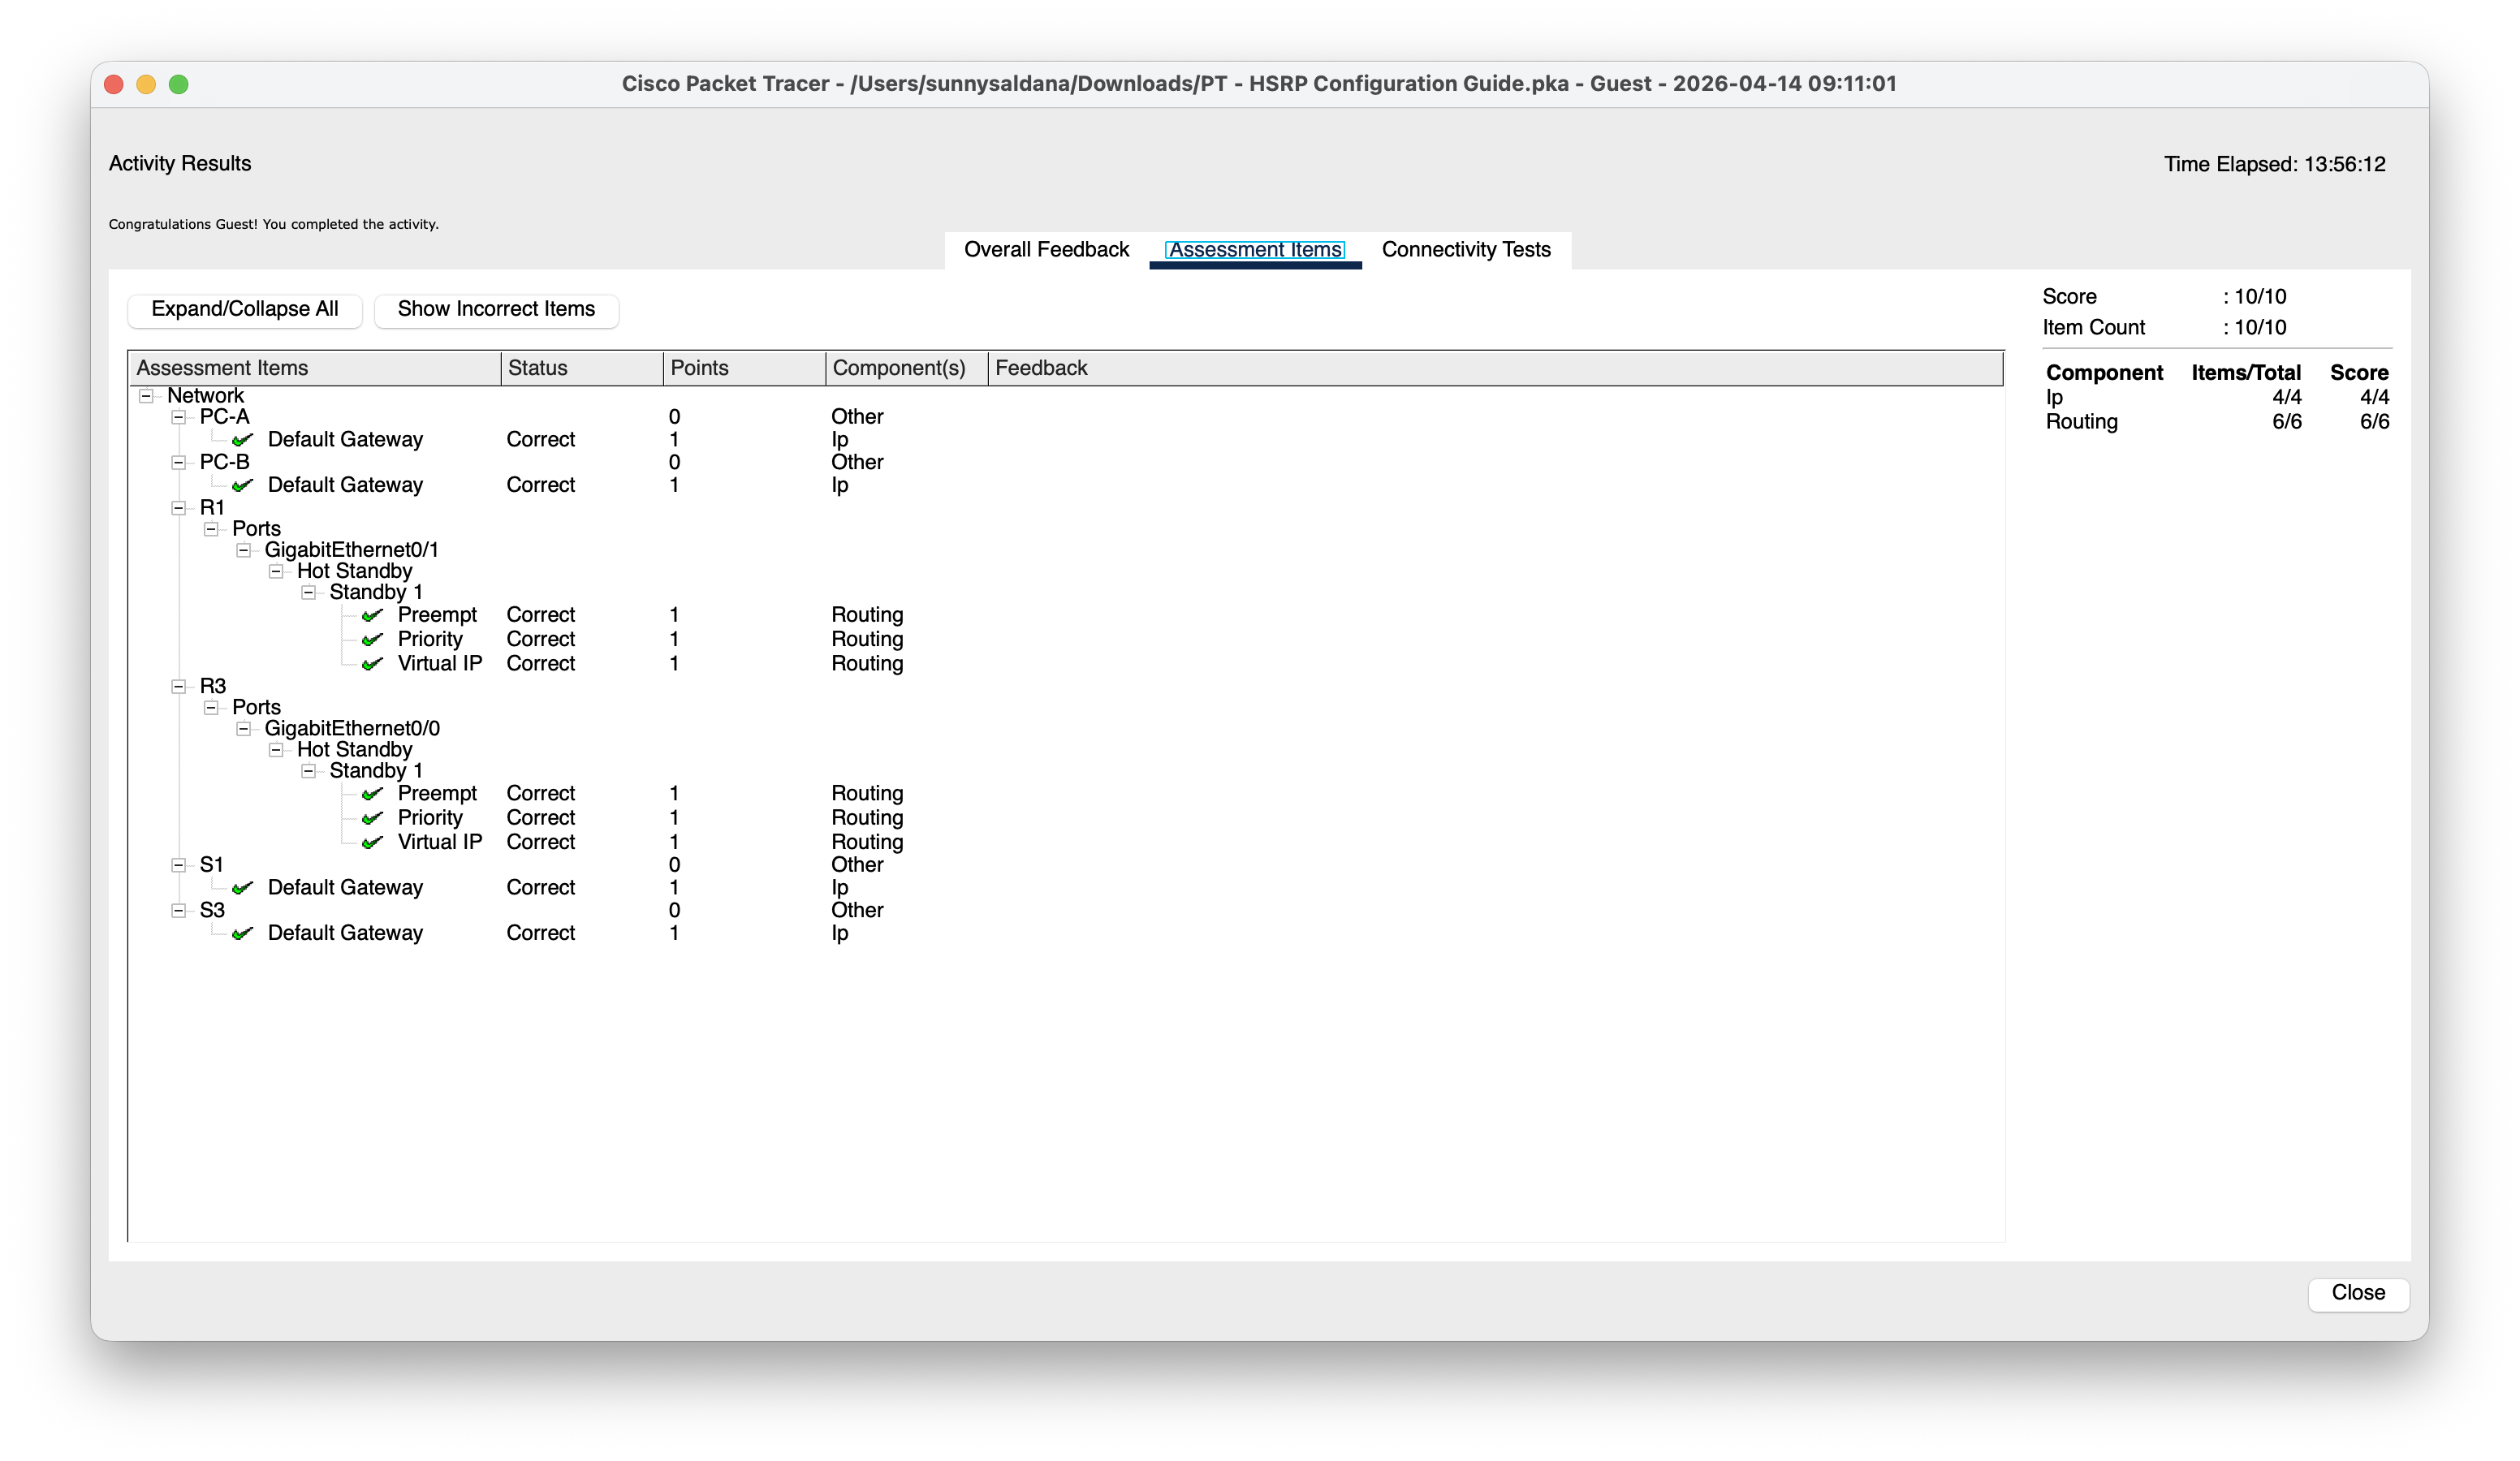
\includegraphics[width=0.8\textwidth]{resultadosResumen.png}
  \caption{Resultados Packet Tracer}\label{fig:resultadosResumen}
\end{figure}

\section{Conclusiones}

HSRP es una solución efectiva para garantizar redundancia en la puerta de enlace predeterminada. Su implementación permite mantener la conectividad de los dispositivos finales incluso ante fallos de infraestructura, mejorando la confiabilidad de la red.

El uso de prioridades y la opción \texttt{preempt} permite controlar qué router debe operar como activo, optimizando el flujo de tráfico.

\end{document}